% updated April 2002 by Antje Endemann
% Based on CVPR 07 and LNCS, with modifications by DAF, AZ and elle, 2008 and AA, 2010, and CC, 2011; TT, 2014; AAS, 2016; AAS, 2020

\documentclass[runningheads]{llncs}
\usepackage{graphicx}
\usepackage{comment}
\usepackage{amsmath,amssymb} % define this before the line numbering.
\usepackage{color}

% INITIAL SUBMISSION - The following two lines are NOT commented
% CAMERA READY - Comment OUT the following two lines
\usepackage{ruler}
\usepackage[width=122mm,left=12mm,paperwidth=146mm,height=193mm,top=12mm,paperheight=217mm]{geometry}

\usepackage{amsmath}
\usepackage{amssymb}
\usepackage{mathrsfs}
\usepackage{amssymb}
\usepackage{multirow}
\usepackage{subfigure}
\usepackage{booktabs}
\usepackage{floatrow}
\graphicspath{{pic/}}

% Include other packages here, before hyperref.

% If you comment hyperref and then uncomment it, you should delete
% egpaper.aux before re-running latex.  (Or just hit 'q' on the first latex
% run, let it finish, and you should be clear).
\usepackage[pagebackref=true,breaklinks=true,letterpaper=true,colorlinks,bookmarks=false]{hyperref}


\begin{document}
% \renewcommand\thelinenumber{\color[rgb]{0.2,0.5,0.8}\normalfont\sffamily\scriptsize\arabic{linenumber}\color[rgb]{0,0,0}}
% \renewcommand\makeLineNumber {\hss\thelinenumber\ \hspace{6mm} \rlap{\hskip\textwidth\ \hspace{6.5mm}\thelinenumber}}
% \linenumbers
\pagestyle{headings}
\mainmatter
\def\ECCVSubNumber{242}  % Insert your submission number here

\title{Exploring global point context for 3D detection} % Replace with your title

% INITIAL SUBMISSION 
%\begin{comment}
\titlerunning{ECCV-20 submission ID \ECCVSubNumber} 
\authorrunning{ECCV-20 submission ID \ECCVSubNumber} 
\author{Anonymous ECCV submission}
\institute{Paper ID \ECCVSubNumber}
%\end{comment}
%******************

% CAMERA READY SUBMISSION
\begin{comment}
\titlerunning{Abbreviated paper title}
% If the paper title is too long for the running head, you can set
% an abbreviated paper title here
%
\author{Xu Liu\inst{1}\orcidID{0000-1111-2222-3333} \and
Jian Wang\inst{2,3}\orcidID{1111-2222-3333-4444} \and
Boxin Shi\inst{2,3}\orcidID{1111-2222-3333-4444} \and
Xiaodong He\inst{1}\orcidID{2222--3333-4444-5555}}
%
\authorrunning{F. Author et al.}
% First names are abbreviated in the running head.
% If there are more than two authors, 'et al.' is used.
%
\institute{Princeton University, Princeton NJ 08544, USA \and
Springer Heidelberg, Tiergartenstr. 17, 69121 Heidelberg, Germany
\email{lncs@springer.com}\\
\url{http://www.springer.com/gp/computer-science/lncs} \and
ABC Institute, Rupert-Karls-University Heidelberg, Heidelberg, Germany\\
\email{\{abc,lncs\}@uni-heidelberg.de}}
\end{comment}
%******************
\maketitle

\begin{abstract}
%The abstract should summarize the contents of the paper. LNCS guidelines
%indicate it should be at least 70 and at most 150 words. It should be set in 9-point
%font size and should be inset 1.0~cm from the right and left margins.
\dots
\keywords{3D Point Cloud, Object Detection, Contextual feature}
\end{abstract}


\section{Introduction}
The challenging task of object detection with 3D point cloud plays a key role for Autonomous Driving and Robotics. Previous methods  like \cite{voxelnet} leverage this problem by partitioning the 3D space into regular sized voxels or transforming into the BEV(Bird Eye View) \cite{pixor} and then apply the conventional CNN methods.
However, the initial quantization process of these methods will inevitably introduces the quantization error and this may inhibit the performance of the algorithm.

Recently, the PointNet/PointNet++ \cite{pointnet,pointnet++} has shed lights  on modeling the 3D point clouds directly from the raw-input, thus the quantization error can be avoided. The PointNet++ utilized a series  of Set Abstraction or SA operators to enlarge the receptive field gradually and obtain global information. This merit has enabled  VoteNet\cite{VoteNet} and PointRCNN \cite{PointRCNN} to achieve  state-of-the-art performance on prevailing benchmarks like \cite{SUN_RGBD,SCannet}. But the number of point is also reduced by each of SA operation, the loss of information will limit the performance  of  detection. In short, this prevailing  method  seeks to obtain the global information by simply enlarging the receptive field. However, it is not instinctive enough to obtain the global contextual information with this approach. The global information may still be imreachable beyond the range of the largest receptive field. %not intuitive enough 


As shown in Figure \ref{fig:Flyer}, the global contextual clues in the complex indoor scene can help to determine the category of the objects:  the table in the meeting room should be surrounded by the chairs; this  global contextual information and the inherent relationship can make it easy  to determine the category of the object among the long list in Figure \ref{fig:Flyer}).

In the era of statistical learning, the global context of the image/language are obtained intuitively by encoding the statistics of features with the dictionary. Like VLAD\cite{VLAD},BoW\cite{BoW1,BoW2,BoW3,BoW4}, and Fisher Vector \cite{FisherVector1,FisherVector2}. Inspired by such theories, Zhang et al proposed an end-to-end,  differentiable encoding layer \cite{DeepTEN} that encompass the function of dictionary learning and  residual encoding. This design has been proved successful for texture encoding \cite{DeepTEN} and other 2D tasks \cite{encnet,pascal,ImageNet}, thus  motivating us to leverage this design in 2D tasks to exploit the global contextual information in the 3D point clouds. In this work, we utilize this layer to exploit the global context of point cloud for 3D detection.
\begin{figure}[t]
\label{fig:Flyer}
			\begin{minipage}{1\textwidth}
				\centering
				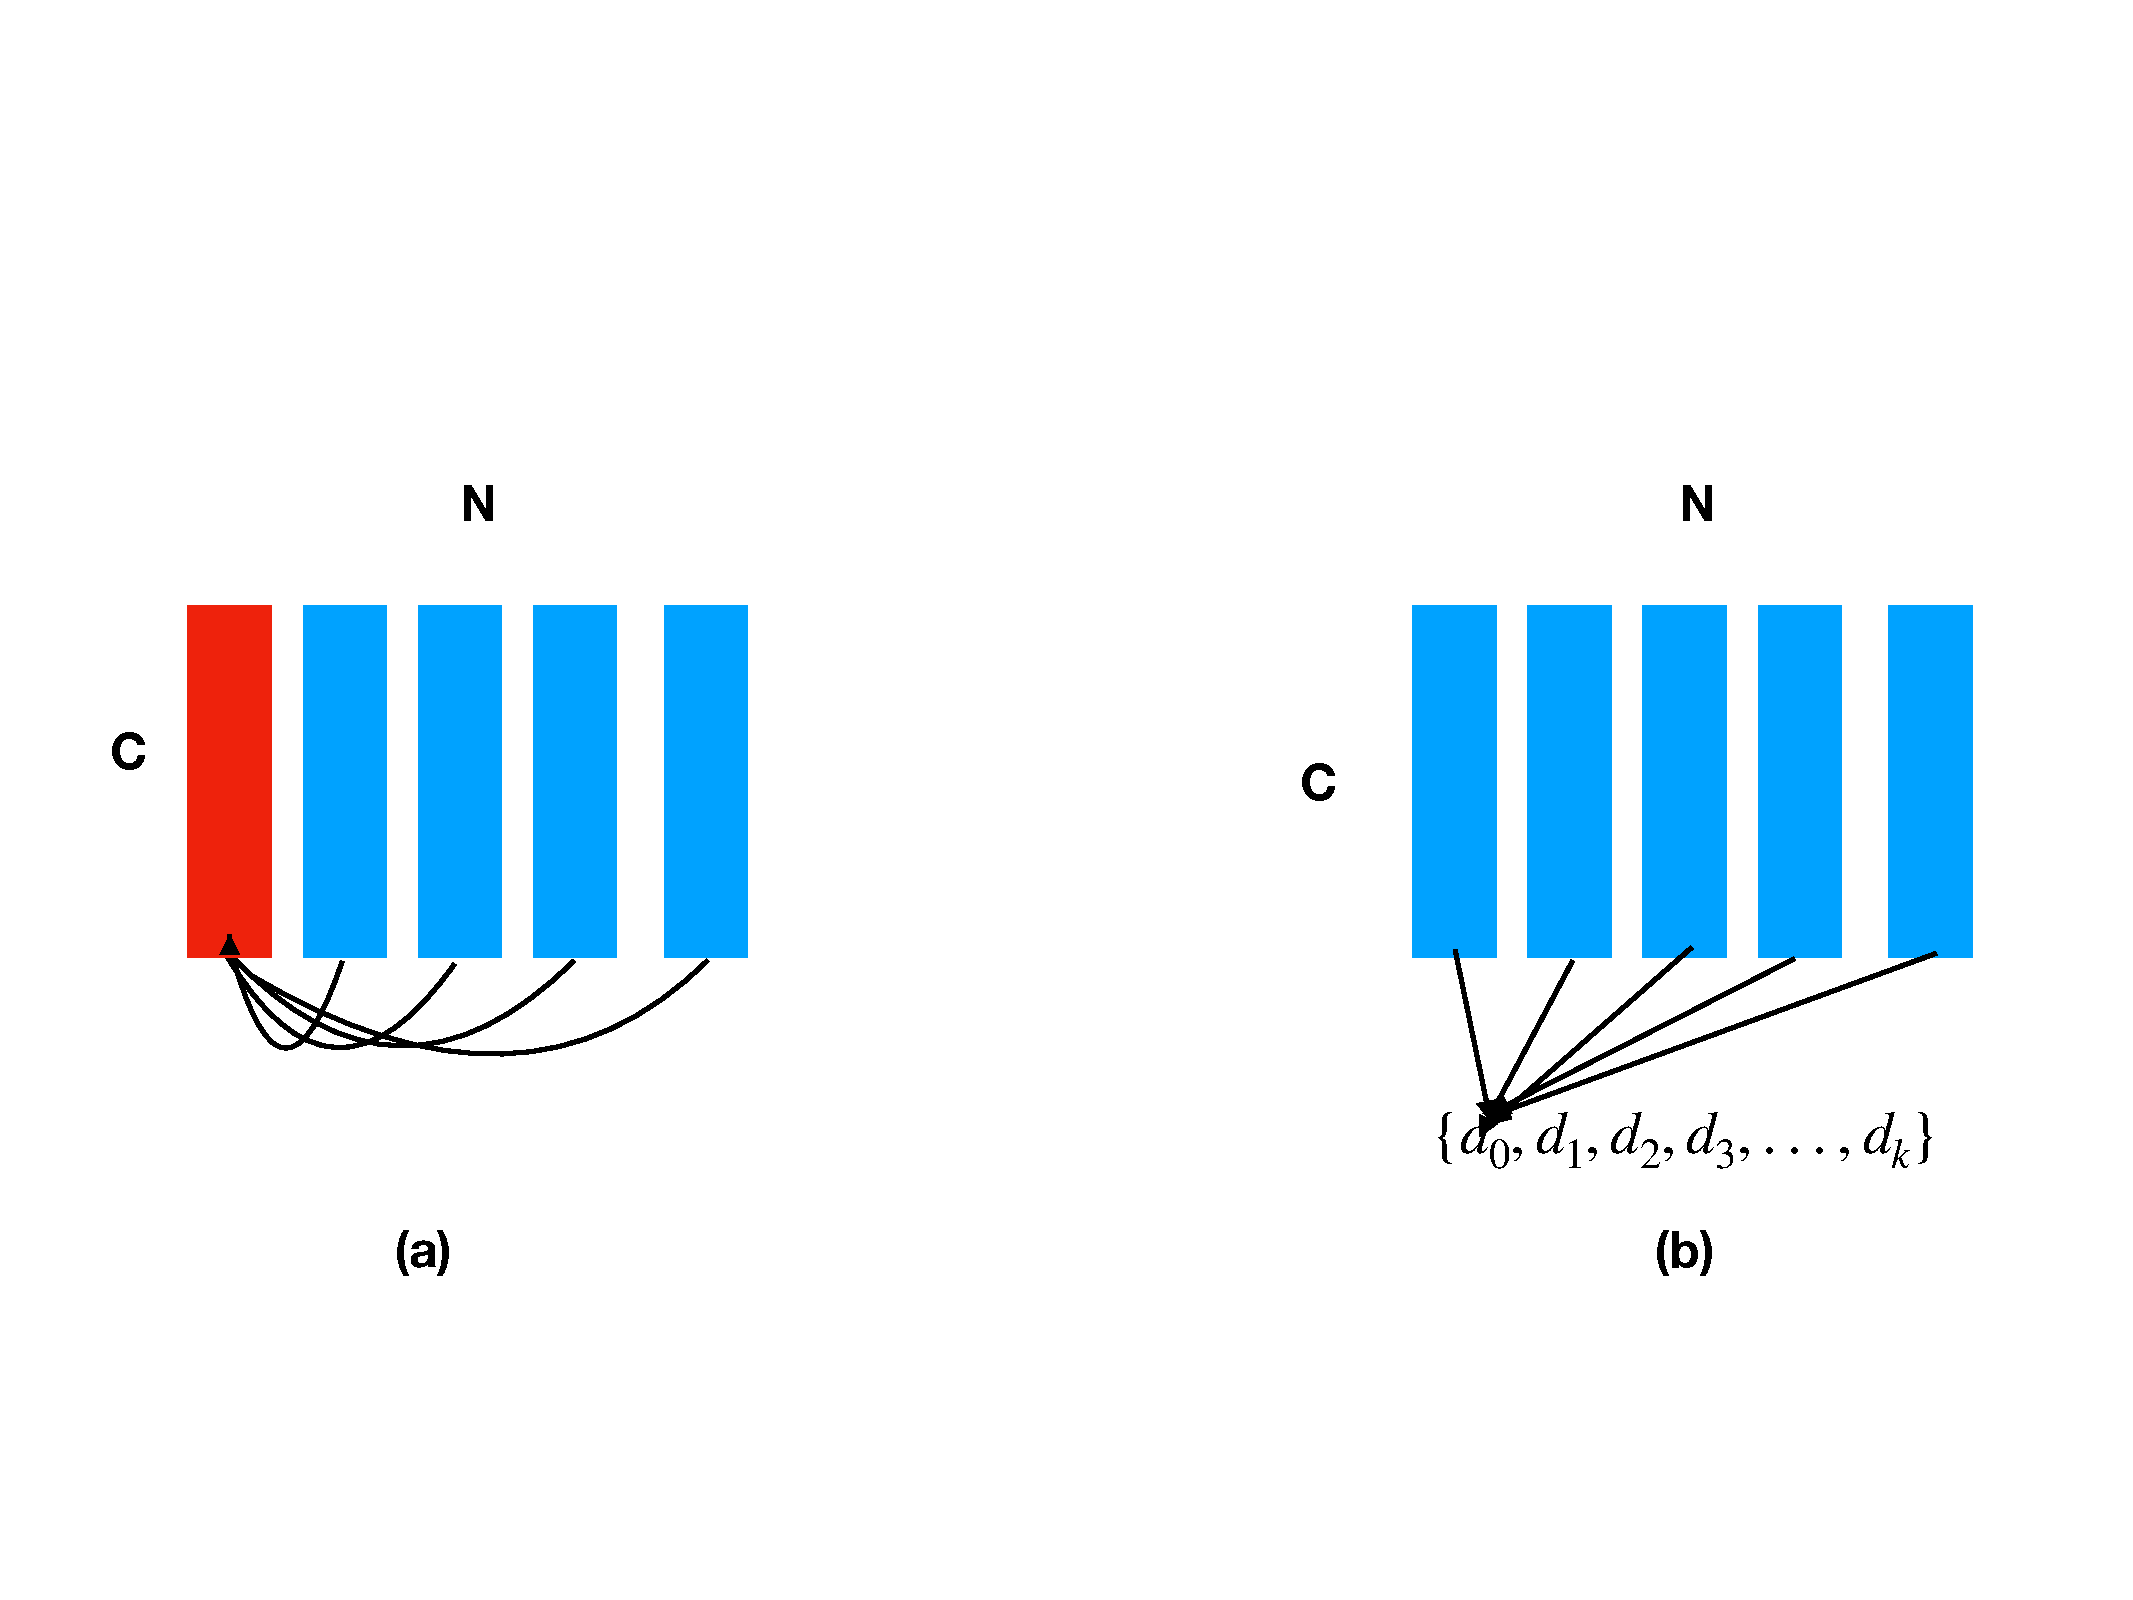
\includegraphics[width=1.1\linewidth]{eccv2020kit/Figure/Flyer.pdf}
			\end{minipage}
    \caption{The contextual priors can be helpful for 3D detection task: the table in the meeting room shown by Figure \ref{fig:Flyer}  should be surrounded by the chairs, this relationship can narrow down the choice among the list. Making it easier for the network to choose the correct label.}
    
\end{figure}
 
The contributions of our paper are in the following aspects:
\begin{itemize}
    \item %We are the first attempting to capture the global context of point cloud for 3D detection. To achieve this goal, 
    We proposed the \emph{Point Contextual Encoding Module} by incorporating the Encoding Layer to capture global information of the point sets, then use this information to modulate the channel-wise embedding of the Point Set features. So that it can highlight or de-emphasize the featuremap  according to the global contextual priors.
    
    \item  By utilizing the  \emph{Point Contextual Encoding Module}  as the building block and following the design of PointNet++ , and the feature representation has been improved by the global contextual information  \emph{Point Contextual Encoding Module}.
 
    \item The experiment has shown  the efficacy and the efficiency of our method.
    
\end{itemize}

\section{Related Works}
\label{related_works}

\noindent{\textbf{PointNet++ Architecture}}

In recent years,  methods \cite{pointcnn,sawnet,relation-shape,ASIS,Graph_Network,kpconv,Pointconv,Geo-CNN,Tangent_Convolution,A-cnn,shape_matching,shapecontextnet} have been proposed to design end-to-end models for point cloud. Pioneering work of PointNet \cite{pointnet} proposes an innovative way to model the raw input data of point sets. Coming after it, PointNet++ \cite{pointnet++}  introduces  Set Abstraction (SA) - Feature Propagation (FP) paired encoder-decoder  structure: The SA operators  will enlarge the receptive field and reduce the point number sequentially in the phase of encoder . Then in the decocder phase, the FP operators are utilized to recover the point number and fuse the skip-connected features of different layers. This structure lacks the ability to acquire global context effectively.

\noindent{\textbf{Context in 3D point clouds}}

To explore the relationships between the  points, Zhao et al. proposed the \cite{pointweb} to exploit the local context among the neighbours. This method has its limitation to obtain the global context of the entire scene.

\cite{ppfnet} and  \cite{LG-PointNet++} is pioneering in obtaining global context for 
point cloud segmentation.  But the global feature is computed by scanning each pair or local patches intensively, which is computational expensive for the dense-clustered indoor scenes.


In comparison with our method,  the global context is computed by encoding with only a few numbers of code words in the dictionary of the encoding layer, which is computational economical.



\noindent{\textbf{PointNet++ based detectors}}

The current detectors  \cite{VoteNet,PointRCNN,STD} typically adopt PointNet++  mentioned above as the backbone to model the raw input of point clouds. Among these detectors, PointRCNN \cite{PointRCNN} and STD \cite{STD} can be classified into the category of \emph{two-stage} detector, %of their bottom-up proposal generation network in the first stage. 
while VoteNet \cite{VoteNet} is a \emph{one stage} single shot 3D detection network. 


\noindent{\textbf{Context in 2D}} 
%\subsection{Context in 2D}

Methods of \cite{Deeplabv1,Deeplabv3,Deeplabv3+,DenseASPP,largekernel,SENet,encnet} in 2D introduce efficient ways of multi-scale contextual feature aggregation and some of the methods has been leveraged for  3D problems.


\begin{figure}[t]
			\begin{minipage}{1\textwidth}
				\centering				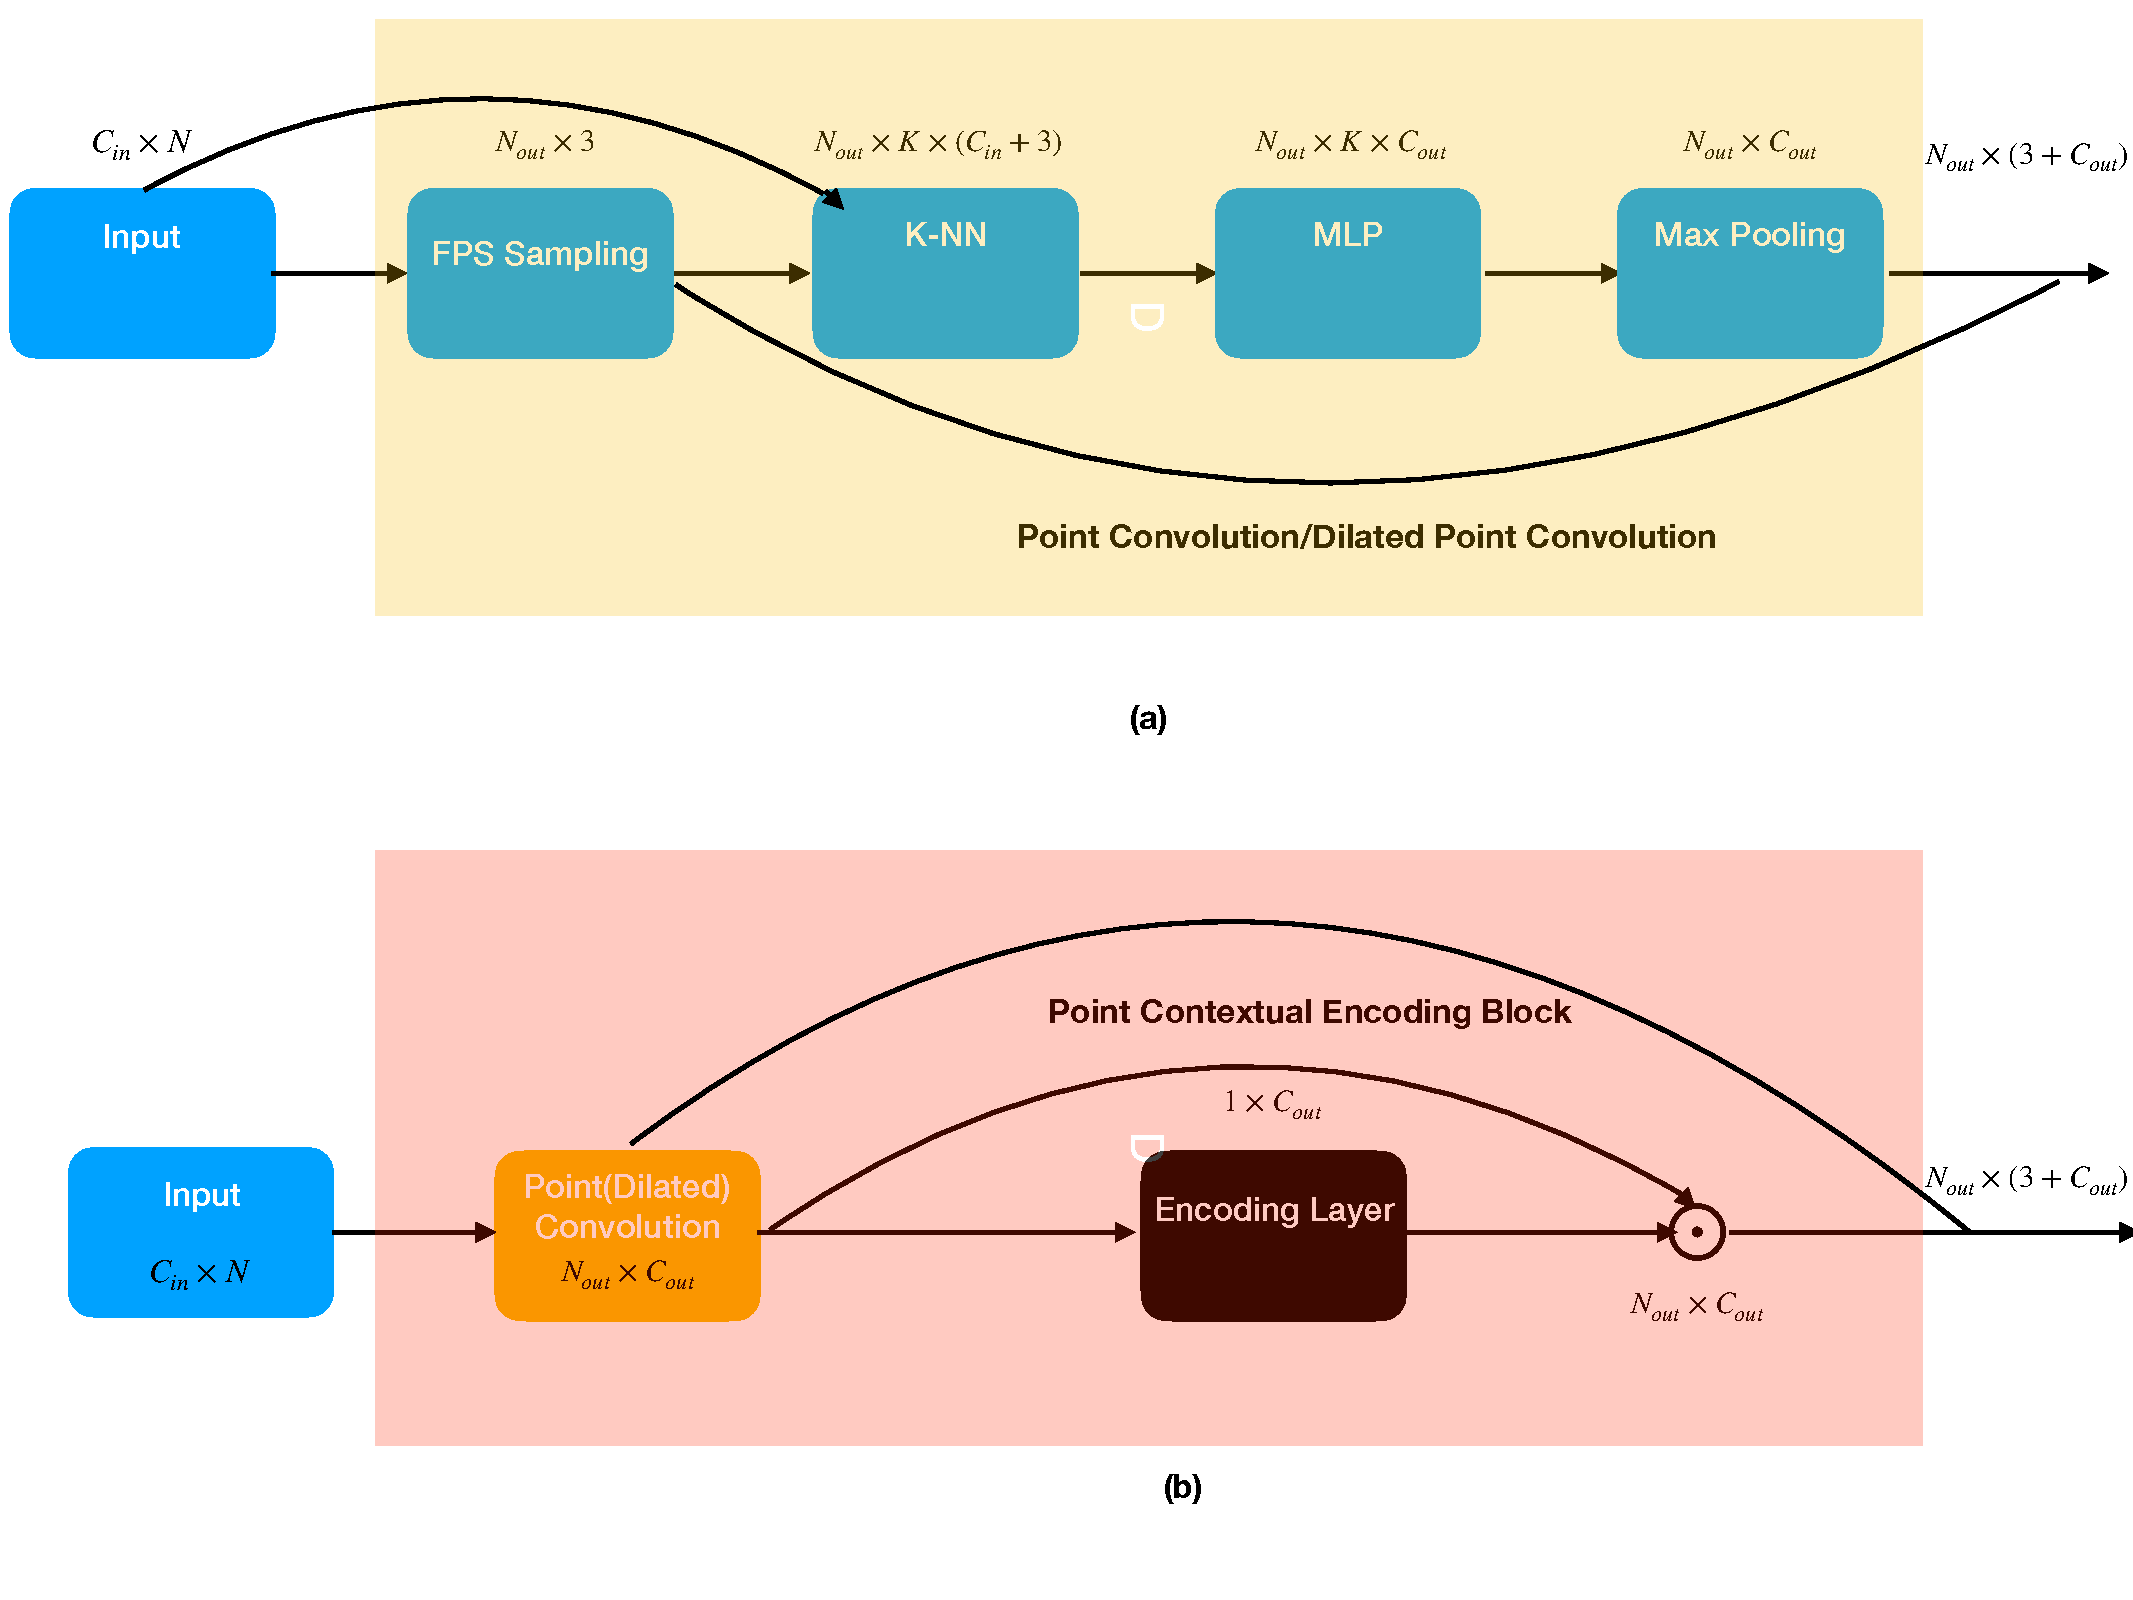
\includegraphics[width=1.0\linewidth]{eccv2020kit/Figure/SA_layer.pdf}
			\end{minipage}
    \caption{The comparison of Point Convolution (a) and Point Contextual Encoding Block(b)}
    \label{fig:PointConv}
\end{figure}

\section{Interpretation of PointNet++ with Point Convolution}

The PointNet++ \cite{pointnet++} consists of a series of SA( Set Abstraction) layers to extract the features. The procedure of the SA layer is illustrated in Figure \ref{fig:PointConv} (a): with the given point set and the feature, it uses the Farthest Point Sampling (FPS) strategy to sub-sample the output points from the input. %and determine the output points. 
Then for each of  the sampled point, the K-NN method is applied to choose the features from the K nearest points. Then the new feature will be computed by passing the information of k points  to a MLP (Multi-Layer Perception) network, a max pooling operator is then appended to reduce the size and then finally concatenate the feature with the coordinates of the output points.

This process can be also formulated by Point Convolution in the followings:

\noindent \textbf{Point Convolution} 
For the point sets, the feature map $X$ is yield by  
\begin{equation} 
X= (f*g)(x)= \sum_{x_{i}\in N_{x}} g(x_{i}-x)f_{i} \label{equation:PointConv}
\end{equation}
where we dub $x_{i}$ as coordinate of the point and $f_{i}$ as its corresponding input feature ,  $g$ is kernel of the convolution.  $N_{x} = \left\{  \left\|x_{i}-x  \right\| \leq r \right\}$ is the set of the points chosen by neighbourhood within certain radius $r$.

In practice, the points of $N_{x}$ are sampled by $k$ nearest neighbours (kNN). And the the kernel $g(x)$ is the Multi-Layer Perception network, denoted by $g(x)=MLP(x)$. This procedure is depicted on Figure \ref{fig:PointConv} (a). and Equation \ref{Equa:PointConv} and \ref{Equa:MLP}.

And the $\theta$ is the hyper parameter of MLP layer. 

\begin{equation}
    X = (f*g)(x) = \sum_{i=1}^{i=k}g(x_{i}-x)f_(x_{i})
    \label{Equa:PointConv}
\end{equation}

\begin{equation}
    g(x) = MLP_{\theta}(x)
    \label{Equa:MLP}
\end{equation}






\section{Method}

\subsection{The importance of Global Context}
\label{sec:bayesian}
The statistics of the  point cloud in the  high-dimensional feature space can be exploited for better  feature representations. We assume this  distribution  on individual point $x$ of the scene $\Omega$ can be represented by $P(x,\Omega)$. 

However, this idealistic distribution is difficult to estimate . In practice,  the conditional statistics or Probability $P(x|\Omega)$  of the scene $\Omega$ is used  for estimating the  distribution.  The softmax normalization operator widely used in deep neural networks to obtain probability logit for criterion can be regarded an example of  $P(x|\Omega)$.

According to the  Equation \ref{equation:bayesian}, to approximate the value of $P(x,\Omega)$, the statistics of the scene $P(\Omega)$ should be taken into consideration and this is referred to as the global context.
\begin{equation}
   P(x,\Omega) = P(x|\Omega)\times P(\Omega)
   \label{equation:bayesian}
\end{equation}

The global context $P(\Omega)$ should be multiplied with the conditional distribution $P(x|\Omega)$ to rectify the bias. 

This principle %serves as  the guideline for our n introduced in Section \ref{section:method} to
motivates us to introduce the global context in Section \ref{section:method} and combine with this information via  the $\times$ operation.
%re-calibrate the features by multiplying the feature with the global context.

\subsection{Point Context Encoding Block}

In this part, we introduce the  method  to yield  the global context with Point Contextual Encoding layer. As mentioned in section \ref{sec:bayesian}, this layer will be applied to  
the Point Convolution operator and the global context will be multiplied with the original feature of the Point Convolution so that it will be empowered by the global context and lead to better performance. 


As shown in Figure \ref{fig:PointConv} (b), this is dubbed as the Point Context Encoding block, and this constitutes the backbone in our design. 

\label{section:method}

\noindent \textbf{Point Contextual Encoding Layer}

% The contextual information of the point sets is crucial for the task of 3D object detection. 
To capture the global contextual feature of the point sets. We leverage the encoding layer in \cite{DeepTEN} to exploit the statistics of the point sets. The encoding layer learns the codebook spontaneously and then encode the features according to  the  residual between the feature and the code words. The global contextual prior will be then be multiplied for re-calibrating the featuremap.

For the feature $X \in \mathbb{R}^{ C \times N}$ $X=\left\{ X_{1} ... X_{N}\right\}$  of the point sets, where $N$ is the number of the point sets and $C$ is the channel number.Let 
the code book $D=\left\{d_{1},d_{2},...d_{K} \right\}$ has $K$ code words to be learned by the network.

The residual will be weighted summed by $e_{k}=\sum_{i=1}^{N} e_{ik}$
\begin{equation}
e_{ik} = \frac{e^{-s_{k}\left\| r_{ik}\right\|^{2}}}{\sum_{j=1}^{K} e^{-s_{k}\left\| r_{ik}\right\|^{2}} r_{ik}}
\label{encoding}
\end{equation}

And the residuals are given by $r_{ik}= x_{i}-d_{k}$. The scaling factor $s$ is a learn-able parameter in the process.
To obtain the global context of the scene, the information of the encoders will be aggregated by the sum operation after passing each  of the encoders individually with Batch Normalization \cite{BN} and ReLU operations,denoted with $\phi$,  which is given by
\begin{equation}
    e=\sum_{i=1}^{K} \phi (e_{k})
 \label{aggregation}  
\end{equation}

The computation complexity of the whole procedure is $O(N \times K)$ , which is computation economical.

It should also be noted that when $K=0$, the encoding layer is degenerated into global average pooling introduced in PSPNet \cite{PSPNet}.

To make use of the aggregated information $e$, it  will pass through a fully connected layer and sigmoid activation function and be utilized as  channel-wise attention, which is similar to \cite{SENet}.  This process is given by $\gamma=\sigma(We)$, where the $\sigma$ denotes for the sigmoid activation, and $W$ stands for the weight of the FC (Fully Connected) layer.

The global descriptor $\gamma$ will be multiplied with the input feature $X$ with the channel wise multiplication: $Y=X\odot \gamma$ for it acts as modulator  of the featuremap: For instance, it will de-emphasize the probability that the furniture appears in the bathroom. And will increase the likely-hood that the pillow that appears on the bed according to the global context obtained from the encoding layer. 
\label{sec:PointEnc}


\subsection{Enc-PointNet++}
The structure of our model is homogeneous with PointNet++ \cite{pointnet++}. It followed the encoder-decoder design which pass through a series of Point Contextual Encoding Blocks in section \ref{sec:PointEnc}, then in the decoder phase, the feature will be up-sampled , fused and  recovered back to its original size. 

\begin{figure}[t]
\begin{minipage}{1.0\textwidth}
    \centering
    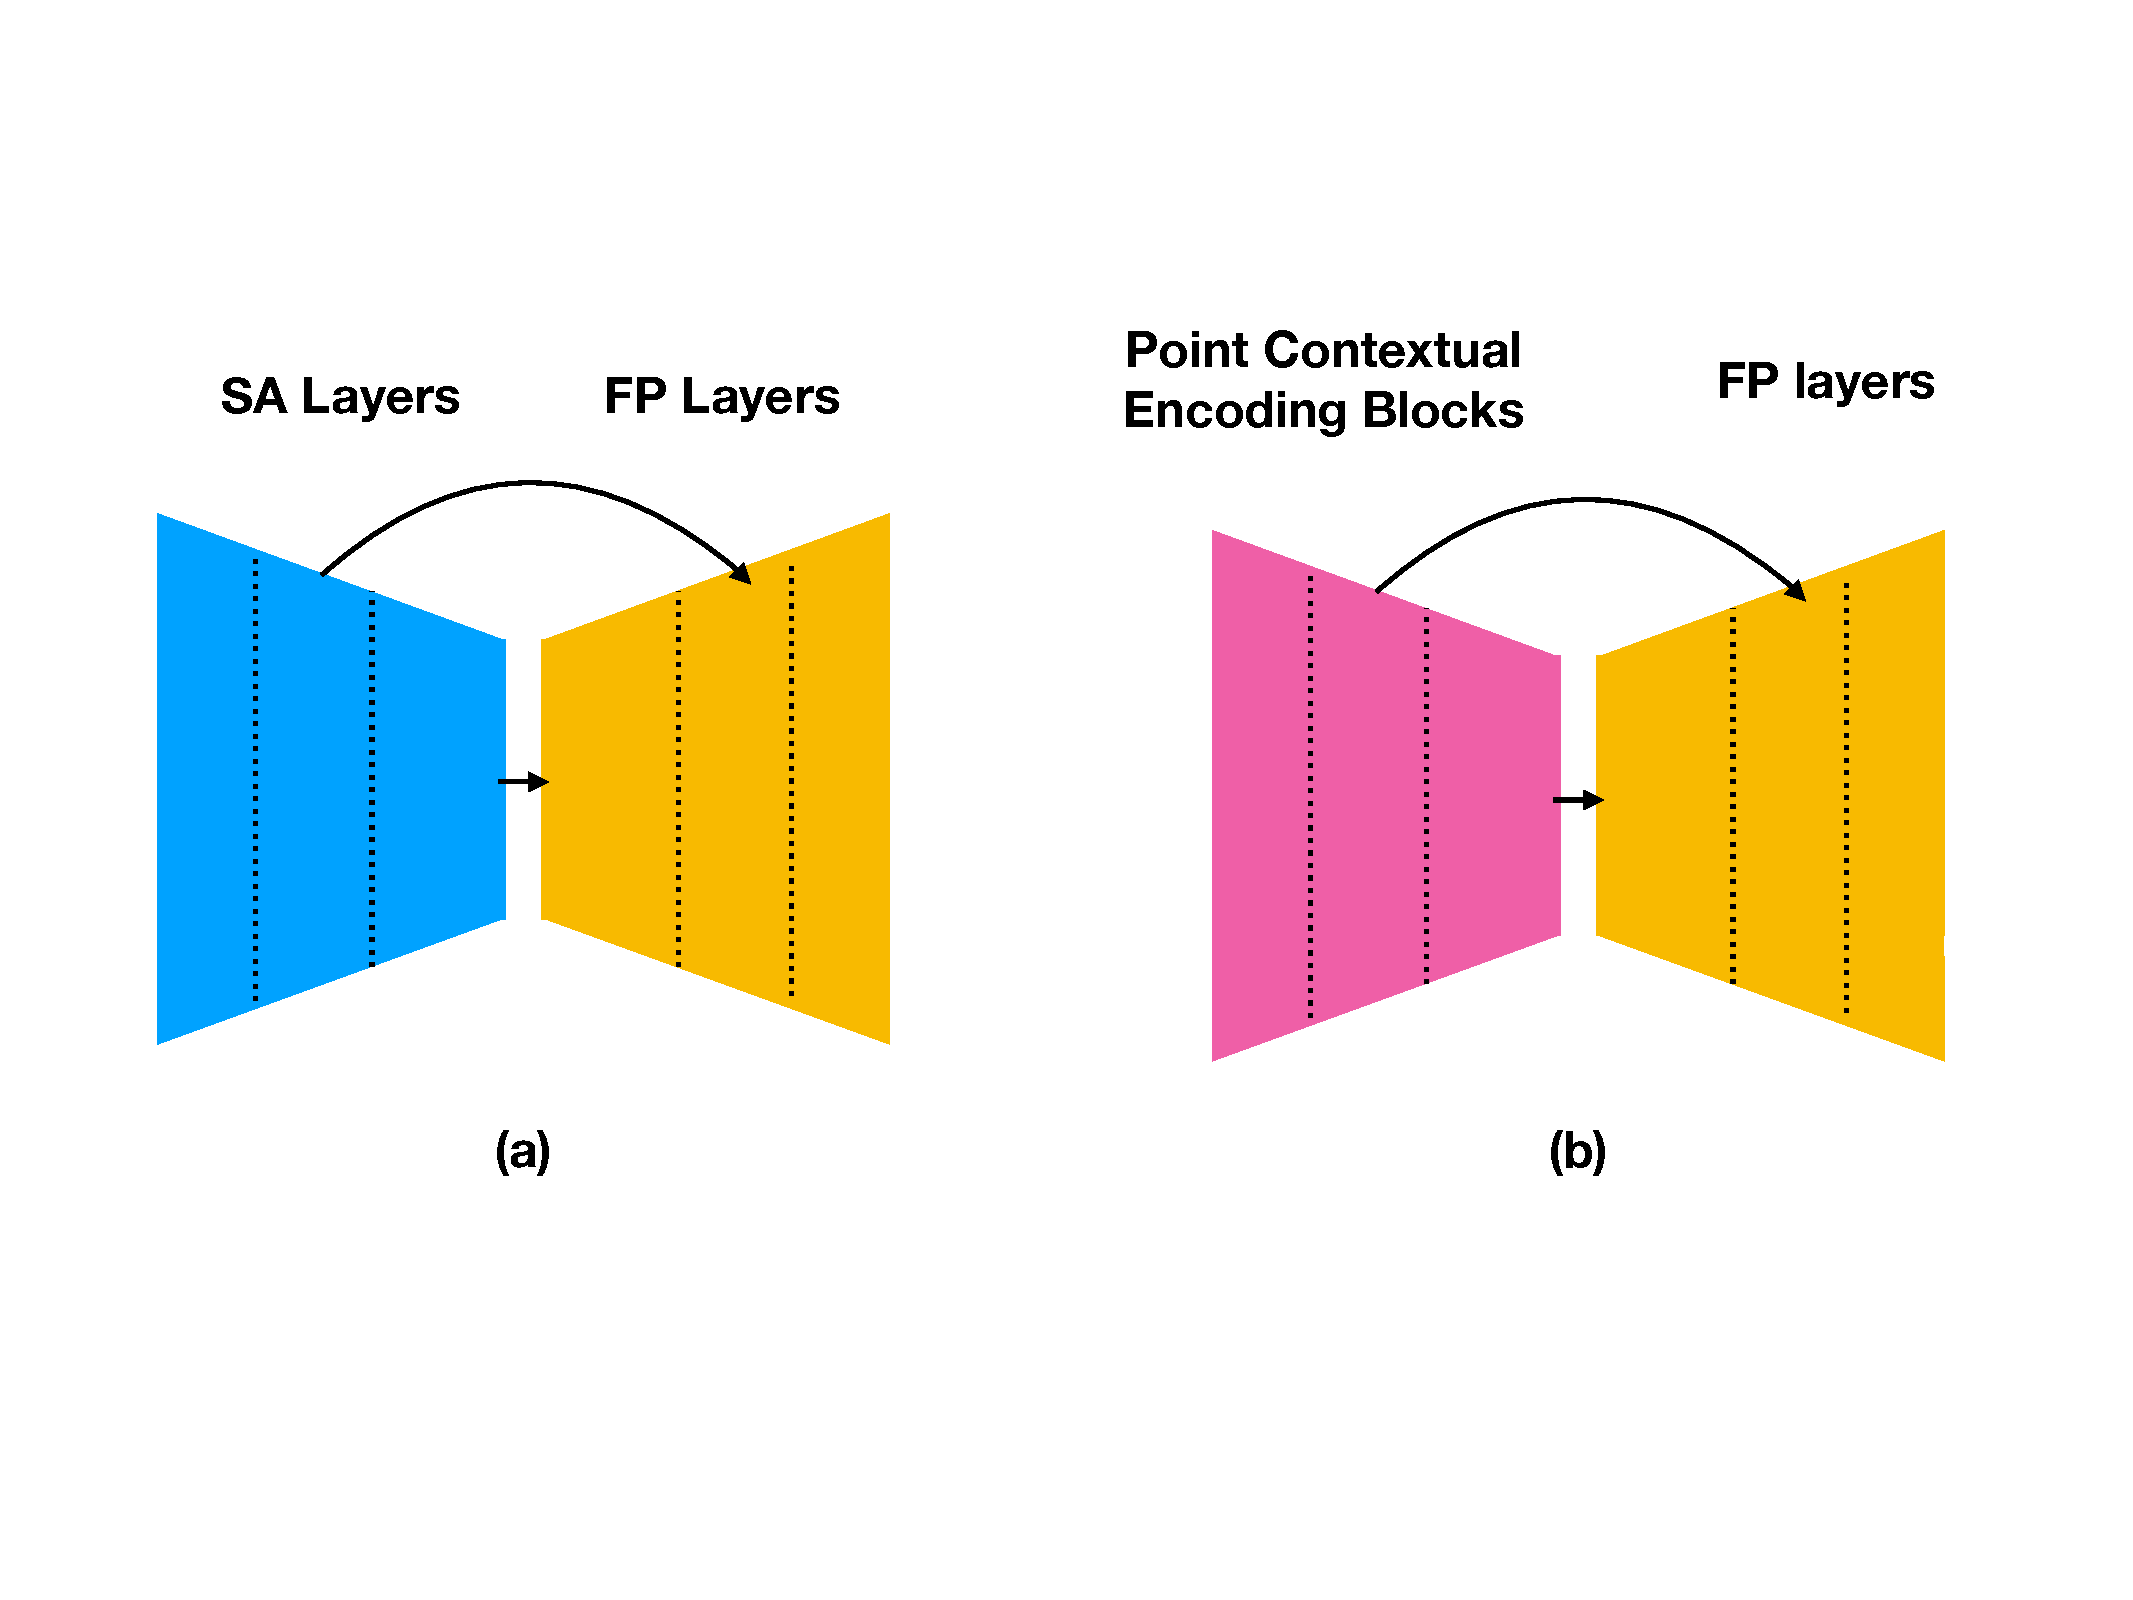
\includegraphics[width=.8\linewidth]{eccv2020kit/Figure/enc_pointnet++.pdf}
    \caption{The structure of PointNet++ in (a) and our Enc-PointNet++ in (b) }
\end{minipage}
\label{fig:enc_pointnet}
\end{figure}

In contrast with the original PointNet++, the feature from each of the SA layers will be enhanced by the global context within its range of scale.  Therefore, the Enc-PointNet++ should be more powerful than its counterpart of PointNet++.

\begin{figure}[t]
\begin{minipage}{1.\textwidth}
    \centering
    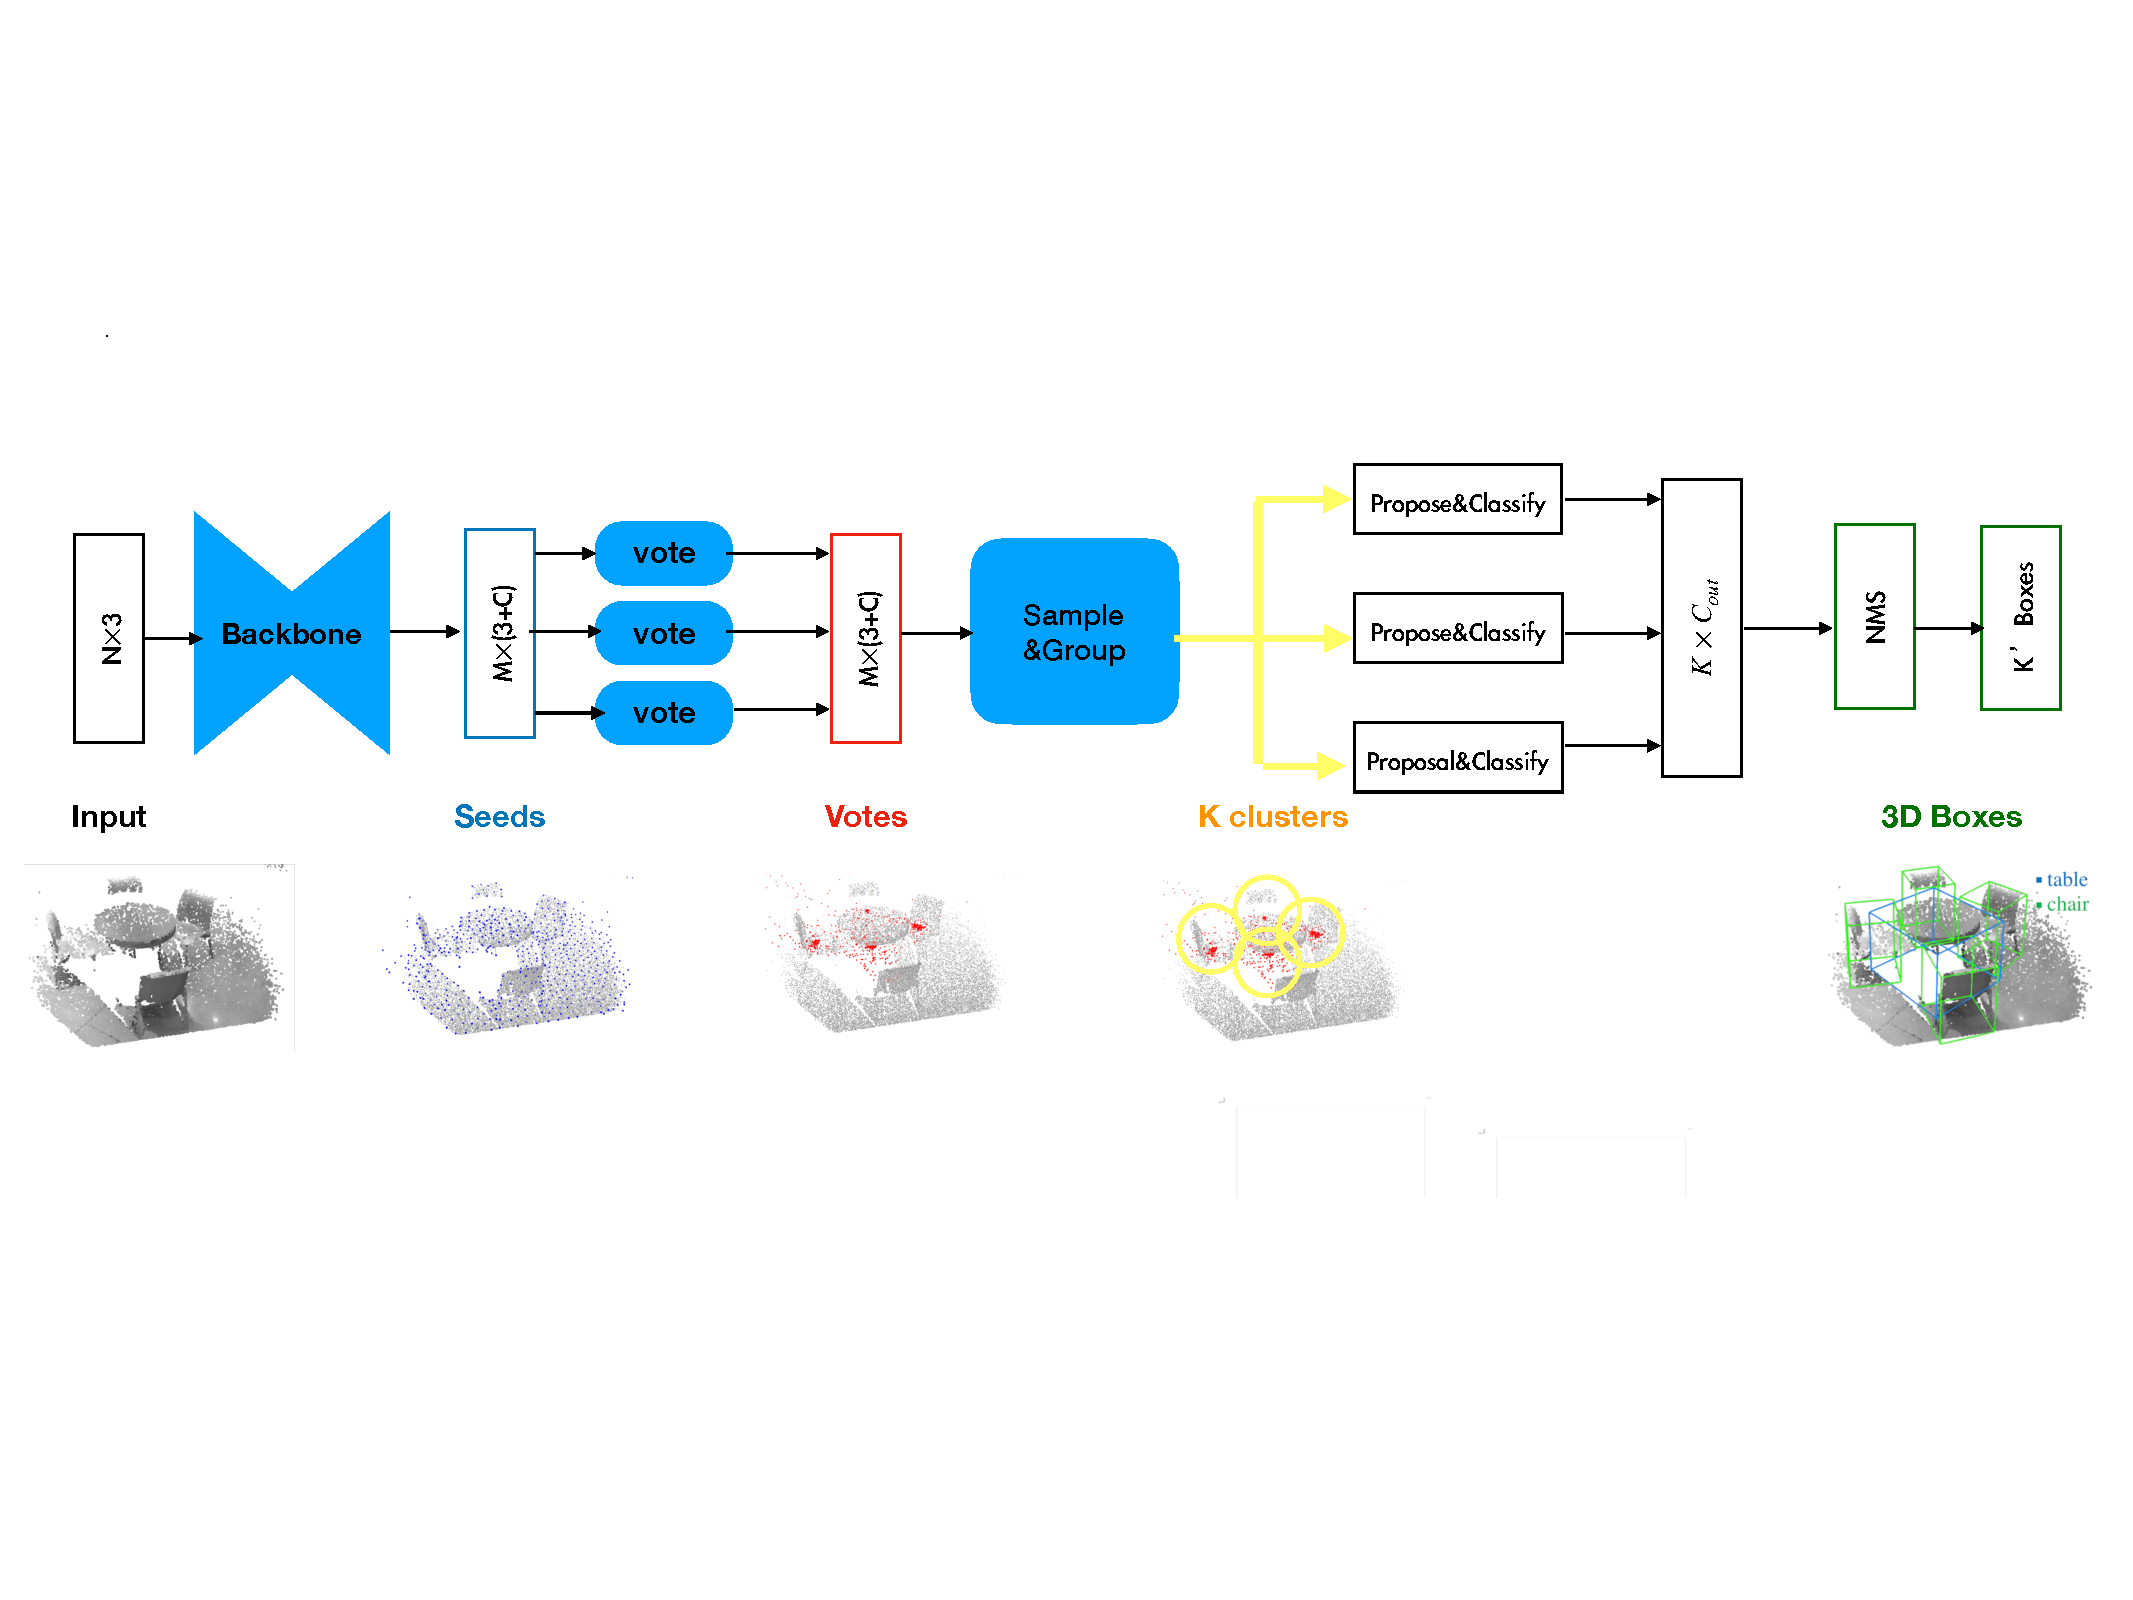
\includegraphics[width=1.0\linewidth]{eccv2020kit/Figure/VoteNet.pdf}
    \caption{VoteNet}
\end{minipage}
\label{fig:votenet}
\end{figure}


This backbone will be plugged on the VoteNet \cite{VoteNet}
The procedure of Votenet is depicted in Figure \ref{fig:enc_pointnet}. The features of the point set will be extracted by the Backbone Network. The points in the seeding layer will then be clustered and grouped into 3D boxes. The box will be further refined by the post-processing NMS method.

\section{Experiments}
\label{section:experiment}
In this section, we first conduct a series of ablation studies to verify the efficacy of our module. 

\subsection{Dataset}
SUN RGB-D \cite{SUN_RGBD} for 3D indoor scene understanding consists of around 10k RGB-D images annotated with 64,595 oriented 3D bounding boxes for nearly 40 object categories. In our experiment, following \cite{VoteNet} we split the training/testing set and report 3D detection performance on the 10 most common categories. 

ScanNet \cite{SCannet} provides a wider range of indoor scenes with more densely scanned objects compared with the SUN RGB-D dataset. We use the  1205 scans for training  and 312 scans  for  testing, respectively.  Vertices from meshes  are sampled as the input point clouds. Following the ground-truth annotation mentioned in \cite{VoteNet}, we predict axis-aligned 3D bounding boxes in these scenarios.

In experiments, we follow the same protocol in \cite{VoteNet} and use the metrics, mean average precision (mAP), at IoU threshold 0.25 for evaluation.

\subsection{Implementation Details} 
\noindent\textbf{Architecture}
We  follow the detection architecture proposed in VoteNet \cite{VoteNet}, as shown in Figure \ref{}, which could be further divided into three key components, noted as  backbone, voting and proposal module. For fair comparison, the configuration of voting and proposal module are kept unchanged. 
 

\noindent\textbf{Training and Inference}
 We adopt the same data augmentation methods with VoteNet \cite{VoteNet} .  Here we also adopted the same optimizer, Adam Optimizer \cite{adam} is utilized with an initial learning rate 0.001. Learning rate is scheduled to be decayed by the factor of 0.1 after 80 epochs and another 0.1 after 120 epochs. There are 180 epochs in total, which is the same with VoteNet\cite{VoteNet}. The whole model is trained on a single Titan X GPU.
During evaluation stage, we take the points of the entire scene as the input. With a \emph{single shot pass}, the region proposals are generated by the neural networks and further post-processed by 3D NMS method.

\subsection{Ablation Studies}
We set a  series of ablation studies and investigate the relationship of performance with the code word number K, and the stage number,  which is shown in the table XXXX. %between the including the relation ship with 

To verify the efficacy of our method, we chose the  SA2 layer as input feature for comparison because this configuration achieved the highest performance in XXX V1. %with VoteNet \cite{VoteNet} and XXX v1, we choose the same configuration with VoteNet \cite{VoteNet} and V1, for instance,
in the table, the \emph{SA2'} means that the point contextual encoding block shares the same hyper-parameters  with SA2 layer in VoteNet\cite{VoteNet} and XXXXX v1. (It should be noted that the SA1 layer is also replaced with point contextual encoding block sharing the same configurations with SA1 as well, ). The SA2'+ Dense Point Diffusion V2(3,6,12)  is constructed by replacing all the Point convolution (SA) operators and Dilated Point Convolution operators of SA2+Dense Point Diffusion(3,6,12) XXXX with the corresponding point contextual encoding blocks. And the code numbers $K$ of each layer are also the same for simplicity.









\noindent{\textbf{Code word number: K}}

To verify the choice of codeword number K in the dictionary, we conducted experiment on SA2' with a series  of numbers K=0,16,32 (The code word of SA1' is the same with SA2') and the results are shown in Table \ref{tab:codeword}.       

The result shows that the the improvement of global average pooling (K=0) is limited, only 0.5 mAP improvement on ScanNetV2 compared with the baseline SA2 , which implies that the operator of global average pooing does not work well for the irregular 3D point clouds.


In theory,  the performance will increase with the code number $K$ because the  complex scenes can be encoded by more independent code words . In practice, we find the performance get saturated when $K=32$. Therefore, we choose the $K=32$ for the following experiments.

\setlength{\tabcolsep}{4pt}
\begin{table*}
\centering
\scalebox{0.8}
{
\begin{tabular}{ccccc}
				\toprule
				\multicolumn{2}{c}{\multirow{3}*{Method}} & \multicolumn{3}{c}{mAP@0.25} \\ %\multicolumn{2}{c}{\multirow{3}*{)}}\\
				\cmidrule(lr){3-5}
				%\multicolumn{2}{c}{} & \multicolumn{2}{c}{640$\times$360} & \multicolumn{2}{c}{1280$\times$720} & \multicolumn{2}{c}{1920$\times$1080} & \\
				\multicolumn{2}{c}{} & SUN RGB-D V1 & SUN RGB-D V2& ScanNetV2 &\multicolumn{2}{c}{} \\
				%\noalign{\smallskip}
				%\midrule
				\midrule
				\multicolumn{2}{l}{SA2} & 51.2 &54.0 &51.2   \\
				\multicolumn{2}{l}{SA2'(K=0)} & 51.9 &54.2 &51.7 \\
				\multicolumn{2}{l}{SA2'(K=16)} & 54.7 &56.4 &53.1 \\
				\multicolumn{2}{l}{SA2'(K=32)} & 55.0 &56.4 &53.4 \\	
            \bottomrule	
			\end{tabular}}
    \caption{Ablation studies of code word K.}
    \label{tab:codeword}
\end{table*}
%\noindent{\textbf{Large Receptive Field Matters}}
% more stages of dilation helps
Table \ref{tab:ablation_studies} shows the performance of different stages of our module based on the same feature (e.g. SA2 or SA2'). The results verify that in general, increasing number of stages of the module will contributes to better performance. For instance, the performance of SA2'+ Dense Point Diffusion V2(3,6) is 60.9 mAP on the benchmarch of SUN-RGBD V2 , which is a boost of \emph{1.4mAP} compared with SA2'+ Dense Point Diffusion V2(3)  and an increase of \emph{3.5mAP} compared with SA2'.
%Compared with the performance of  SA2 baseline, model with one stage of 3 $\times$ dilated convolution already obtains the boost of 6.2 mAP and 6.0 mAP  for SUN RGB-D V1 and ScanNet V2 respectively while those with two more stages achieve the  improvement up to 7.7 mAP for ScanNet V2.


%\noindent{\textbf{Dense Sampling on Point Sets}}
%As mentioned in Section \ref{sec:method}, Dense Point Diffusion Module has the merit of  sampling point sets efficiently regardless of the density distribution, which is crucial for aggregating features at various scales. In Figure \ref{fig:vis-rf}, we show several examples of how the proposed module samples the neighboring points at different stages. With the increasing number of stage involved, the receptive field is expanded steadily and more points will be aggregated for better representation of feature. 


%\noindent{\textbf{Necessity of Dense Aggregation}}
%The good performance of our method may be partially attributed to the cascaded structure of Dilated Point Convolutions. To justify our configuration of the dense module, we degrade our module into the cascaded dilated point convolution with their dilation rates unchanged, noted as PlainNet. Table \ref{tab:additional_experiment} shows this comparison, we notice that performance of the PlainNet drops significantly by  8.2 mAP on the benchmark of SUN RGB-D V1 compared with the  method of Dense Point Diffusion. This suggests that although simply deepening the layer of dilated point convolution helps to increase the receptive field, it fails to improve the overall performance since the range of the feature scale is monotonous compared with  the Dense Point Diffusion module. Therefore, how to efficiently aggregate feature from multiple scales is the key to the success. 
\noindent{ \textbf{Comparison with the Dense Point Diffusion}}
We also make comparisons between Dense Point Diffusion module and V1 XXXX, Point Diffusion Module, with the SA and SA' layer, dense diffusion model v1 and v2 sharing the same configuration of the parameters and dilation rate. The  recalibration of  the  featuremap via the global context of  Point Contextual Encoding module  contribute to better feature representation of the point sets in the scene. As a result, the v2 outperforms the v1 in most of the cases. For example, the performance of SA2'+Dense Point Diffusion V2(3,6) is 60.9 mAP on the benchmark, which is \emph{1.1 mAP} higher than the counterpart of SA2+Dense Point Diffusion(3,6).




%Set Abstraction layers and dilation rates, e.g SA3 + Point Diffusion(3,6) and SA3 + Dense Point Diffusion(3,6). In most cases, performance of the Dense Point Diffusion module is better than the counterpart of the Point Diffusion module, which validates our claims in Section \ref{sec:method}.

To summarize, our module of Dense Point Diffusion V2 inherit  from the advantages  of the XXXX V1,  which can densely aggregate the multi-scale features in the parallel pathways and the cascaded structure of Dilated Point Convolution to gain larger receptive fields. In addition, this module can exploit the global context XXXX in each stage, leading to better performance on the benchmarks.
%thus showing advantages over other modules on 3D detection tasks in complex scenes. 

%\noindent{\textbf{Compact Model Size}}
% Effect of enlarged receptive field
%Results from last column in Table \ref{tab:ablation_studies} keep the track of the parameter number of models. We observe that parameters of Dense Point Diffusion grow in linear relation as the model goes deeper, which is more compact than the conventional backbone utilized in VoteNet \cite{VoteNet}. 


\setlength{\tabcolsep}{4pt}
\begin{table*}
\centering
\scalebox{0.8}
{
\begin{tabular}{cccccccc}
				\toprule
				\multicolumn{2}{c}{\multirow{3}*{Method}} & \multicolumn{3}{c}{mAP@0.25} & \multicolumn{2}{c}{\multirow{3}*{\#Params(MB)}}\\
				\cmidrule(lr){3-5}
				%\multicolumn{2}{c}{} & \multicolumn{2}{c}{640$\times$360} & \multicolumn{2}{c}{1280$\times$720} & \multicolumn{2}{c}{1920$\times$1080} & \\
				\multicolumn{2}{c}{} & SUN RGB-D V1 & SUN RGB-D V2& ScanNetV2 &\multicolumn{2}{c}{} \\
				\noalign{\smallskip}
				%\midrule
				\midrule
				\multicolumn{2}{l}{SA2} & 51.2 &54.0 &51.2 & \multicolumn{2}{c}{0.31} \\
				\multicolumn{2}{l}{SA2'} & 55.0  & 56.4 & 53.4& \multicolumn{2}{c}{XXXX} \\
				%\multicolumn{2}{l}{SA2+Point Diffusion(3,6)} & 58.0 &59.5 & 56.9  & \multicolumn{2}{c}{0.94}\\
				%\multicolumn{2}{l}{SA2+Point Diffusion(3,6,12)} &57.9 & 59.6&  59.0 & \multicolumn{2}{c}{1.26}\\
				\midrule
				\multicolumn{2}{l}{SA2+Dense Point Diffusion (3)} & 57.4 & 59.2& 57.2 & \multicolumn{2}{c}{0.62}\\
				\multicolumn{2}{l}{SA2+Dense Point Diffusion (3,6)} & 58.7 & 59.8&  58.9 & \multicolumn{2}{c}{1.07}\\
				\multicolumn{2}{l}{SA2+Dense Point Diffusion (3,6,12)} & 58.6 & 59.6& 59.6& \multicolumn{2}{c}{1.63}\\

				\midrule
				\multicolumn{2}{l}{SA2'+Dense Point Diffusion V2(3)} & 58.7 & 59.5& 58.2 & \multicolumn{2}{c}{XXX}\\
				\multicolumn{2}{l}{SA2'+Dense Point Diffusion V2(3,6)} & \textbf{59.2} & \textbf{60.9}&  59.3 & \multicolumn{2}{c}{XXX}\\
				\multicolumn{2}{l}{SA2'+Dense Point Diffusion V2(3,6,12)} & 58.8 & 60.3& \textbf{59.8}& \multicolumn{2}{c}{XXX}\\				
				\bottomrule		%\vspace{0.1em}
			\end{tabular}
			}

    \caption{Ablation studies of our module of Dense Point Diffusion and Point Diffusion on different benchmarks with different settings of the baseline feature and module structure.}
    \label{tab:ablation_studies}
\end{table*}


\setlength{\tabcolsep}{4pt}
\begin{table*}
		\begin{center}
			\scalebox{0.75}{
			\begin{tabular}{l|c|cccccccccc|c}
				\toprule
				Method & Input & \rotatebox{90}{bathtub}&\rotatebox{90}{bed}& \rotatebox{90}{book self}& \rotatebox{90}{chair} &\rotatebox{90}{desk}&\rotatebox{90}{dresser}& \rotatebox{90}{nightstand}&\rotatebox{90}{sofa}&\rotatebox{90}{table}&\rotatebox{90}{toilet}&mAP \\
				\noalign{\smallskip}
				\midrule
				\noalign{\smallskip}
				F-PointNet \cite{FrustumPointNet}&Geo+RGB&43.3&81.1&\textbf{33.3}&64.2&24.7&32.0&58.1&61.1&\textbf{51.1}&\textbf{90.9} &54.0 \\
				VoteNet \cite{VoteNet}&Geo Only&\textbf{74.4}&83.0&28.8&\textbf{75.3}&22.0&29.8&62.2&64.0&47.3&90.1 &57.7 \\
				Dense Point Diffusion&Geo Only& 71.9&\textbf{86.3}&30.5&74.1&\textbf{26.3}&\textbf{30.3}&\textbf{63.1}&\textbf{65.2}&49.2&90.3&58.7 \\
				\textbf{Ours}&Geo Only& & & & & & & & & & & \textbf{59.2}\\				
				%&  &  & &  \\
				 %& Res18 & 8.3G & 42.7M & 61.58\\
				\bottomrule
			\end{tabular}}
		\end{center}
		\caption{Comparison with the state of the art algorithm on SUN RGB-D V1 benchmark.}
		\label{tab:SUNRGBD_v1}
\end{table*}

\setlength{\tabcolsep}{4pt}
\begin{table*}
\begin{center}
\scalebox{0.53}{
\begin{tabular}{l|cccccccccccccccccc|c}
\toprule
& \rotatebox{90}{cab} &\rotatebox{90}{bed}&\rotatebox{90}{chair}&\rotatebox{90}{sofa}&\rotatebox{90}{table}&\rotatebox{90}{door}&\rotatebox{90}{wind}&\rotatebox{90}{bkshf}&\rotatebox{90}{pic}&\rotatebox{90}{cntr}&\rotatebox{90}{desk}&\rotatebox{90}{curt}&\rotatebox{90}{fridg}&\rotatebox{90}{showr}&\rotatebox{90}{toil}&\rotatebox{90}{sink}&\rotatebox{90}{bath}&\rotatebox{90}{ofurn}&mAP \\
\noalign{\smallskip}
\midrule
\noalign{\smallskip}
3DSIS Geo \cite{3d-sis}& 12.75&63.14&65.98&46.33&26.91&7.95&2.79&2.3&0.00&6.92&33.34&2.47&10.42&12.17&74.51&22.87&58.66&7.05&25.36\\
VoteNet \cite{VoteNet}&36.27&87.92&\textbf{88.71}&89.62&58.77&47.32&38.10&44.62&7.83&\textbf{56.13}&\textbf{71.69}&\textbf{47.23}&45.37&57.13&94.4&\textbf{54.70}&\textbf{92.11}&37.20&58.65\\
V1\cite{}&\textbf{38.42}&\textbf{89.14}&86.73&\textbf{89.45}&\textbf{62.70}&\textbf{48.62}&\textbf{38.14}&\textbf{49.86}&\textbf{8.03}&51.27&63.11&47.21&\textbf{59.08}&\textbf{69.28}&\textbf{95.78}&51.01&89.36&\textbf{39.42}&59.65\\
\midrule
\textbf{Ours}&& &&&&&&&&&&&&&&&&&\textbf{59.79}\\
				%VoteNet\cite{}&Geo Only&74.4&83.0&28.8&75.3&22.0&29.8&62.2&64.0&47.3&90.1 &57.7 \\
				%\textbf{Ours}&Geo Only& &&&&&&&&&&\textbf{58.7} \\
				%&  &  & &  \\
				 %& Res18 & 8.3G & 42.7M & 61.58\\
\bottomrule
\end{tabular}}
\end{center}
\caption{Comparison of our method with state of the art algorithm on ScanNetV2, evaluated with mAP @0.25.}
\label{tab:SCanNet0.25}
\end{table*}


\setlength{\tabcolsep}{4pt}
\begin{table*}
\begin{center}
\scalebox{0.54}{
\begin{tabular}{l|cccccccccccccccccc|c}
\toprule
%& cab &bed&chair&sofa&table&door&wind&bkshf&pic&cntr&desk&curt&fridg&showr&toil&sink&bath&ofurn&mAP\\
& \rotatebox{90}{cab} &\rotatebox{90}{bed}&\rotatebox{90}{chair}&\rotatebox{90}{sofa}&\rotatebox{90}{table}&\rotatebox{90}{door}&\rotatebox{90}{wind}&\rotatebox{90}{bkshf}&\rotatebox{90}{pic}&\rotatebox{90}{cntr}&\rotatebox{90}{desk}&\rotatebox{90}{curt}&\rotatebox{90}{fridg}&\rotatebox{90}{showr}&\rotatebox{90}{toil}&\rotatebox{90}{sink}&\rotatebox{90}{bath}&\rotatebox{90}{ofurn}&mAP\\

\noalign{\smallskip}
\midrule
\noalign{\smallskip}
3DSIS Geo \cite{3d-sis}& 5.06&42.19&50.11&31.75&15.12&1.38&0.00&1.44&0.00&0.00&13.66&0.00&2.63&3.00&56.75&8.68&28.52&2.55&14.60\\
VoteNet \cite{VoteNet}&8.07&76.06&\textbf{67.23}&68.82&42.36&\textbf{15.34}&6.43&28.00&1.25&9.52&\textbf{37.52}&11.55&27.80&9.96&\textbf{86.53}&16.76&78.87&11.69&33.54\\
%\midrule
XXX \cite{}&\textbf{9.07}&\textbf{83.53}&64.47&\textbf{71.02}&\textbf{44.19}&13.85&\textbf{9.25}&\textbf{32.98}&\textbf{9.88}&\textbf{17.76}&29.69&\textbf{17.00}&\textbf{37.80}&\textbf{13.93}&81.51&\textbf{20.92}&\textbf{80.40}&\textbf{14.37}&35.71\\
\midrule 
\textbf{XXX \cite{}}&&&&&&&&&&&&&&&&&&&\textbf{38.06}\\
\bottomrule
\end{tabular}}
\end{center}
\caption{Comparison of our method with state of the art algorithm on ScanNetV2, evaluated with mAP @0.5.}
\label{tab:SCanNet0.5}
\end{table*}



\subsection{Results on Prevailing Benchmarks}
In this part, we will introduce the performance for the prevailing 3D benchmarks, SUN RGB-D \cite{SUN_RGBD} and ScanNet \cite{SCannet}, respectively. 
\noindent\textbf{SUN RGB-D} The results on the SUN RDB-D V1 are illustrated in Table \ref{tab:ablation_studies}. The performance of SA2' is 55.0 mAP, as we discussed above. With one stage of our module involved, the SA2' + Dense Point Diffusion V2(3) has reached the performance of 58.7 mAP, which is comparable with the best performance of XXXX V1.

The performance still continue to increase with an extra stage involved, with SA2' + Dense Point Diffusion V2(3,6) reached performance of \emph{59.2} mAP. Which is 0.5 mAP higher than the previous state of the art XXXXV1. The comparison with other state-of-the-art method is shown in Table \ref{tab:SUNRGBD_v1}.

Since the scenarios of SUN RGB-D is limited, the receptive field of the module is already big enough when two stages of the module are involved. And more stages does not necessarily  improve the performance, which is similar to the conclusion of XXXV1.  In particular, the performance of SA2' + Dense Point Diffusion V2(3,6,12) is 58.8 mAP, 0.4 mAP less than SA2'+ Dense Point Diffusion V2(3,6).

We can draw similar conclusions on SUN RGB-D V2, and the peak performance is a \emph{60.9} mAP.



\noindent\textbf{ScanNet}  
We deploy our module on a more challenging benchmark of ScanNet, as shown in Table \ref{tab:ablation_studies}. The result shows that the Point Contextual Encoding block is effective even on a more challenging dataset, with SA2' 53.4 mAP on the benchmark and outperforms the SA2 with  2.2 mAP.
The performance of SA2' + Dense Point Diffusion V2(3) and SA2' + Dense Point Diffusion V2(3,6) on ScanNet are 58.2 mAP and 59.3 mAP respectively.

In contrast with SUN RGB-D, the performance of our module still increases with the third stage involved. The performance is 59.8 and the details is shown in Table \ref{tab:SCanNet0.25}. Compared with the counterpart of SA2 + Dense Point Diffusion (3,6 ,12) in XXXXV1, the improvement by the module seems to be slight, with only 0.15 mAP increase in the performance. But on a stricter evaluation metrics of mAP @ 0.5 IoU, the performance of SA2' + Dense Point Diffusion V2(3,6,12)  has reached the 38.0 mAP, which is 2.3 mAP higher than SA2 + Dense Point Diffusion (3,6 ,12) in Table \ref{tab:SCanNet0.5} . The comparison with other methods are also listed in Table \ref{tab:SCanNet0.5} that our method has outperformed the VoteNet \cite{VoteNet} with 4.5 mAP. The result has shown it clearly that our method is better suited for challenging scenarios and high performance 3D detection tasks.
\section{Conclusions}

%The paper ends with a conclusion. 


\clearpage\mbox{}Page \thepage\ of the manuscript.
\clearpage\mbox{}Page \thepage\ of the manuscript.

This is the last page of the manuscript.
\par\vfill\par
Now we have reached the maximum size of the ECCV 2020 submission (excluding references).
References should start immediately after the main text, but can continue on p.15 if needed.

\clearpage
% ---- Bibliography ----
%
% BibTeX users should specify bibliography style 'splncs04'.
% References will then be sorted and formatted in the correct style.
%
\bibliographystyle{splncs04}
\bibliography{egbib}
\end{document}
